\documentclass{article}
\usepackage{amsmath}
\usepackage{amssymb}
\usepackage{graphicx}
\usepackage{tikz}
\usepackage{pgfplots}
\usepackage{float}
\usepackage{subcaption}
\usepackage{geometry}

\geometry{a4paper, margin=1in}

% Define example environment
\newenvironment{example}[1]{
    \begin{trivlist}
    \item[\textbf{Example:}] #1
    \vspace{0.5em}
}{
    \end{trivlist}
    \vspace{1em}
}

\pgfplotsset{compat=1.18}
\usetikzlibrary{patterns,decorations.pathreplacing}

\title{Lecture 9 Examples}
\author{Signals and Systems Course}
\date{}

\begin{document}

\maketitle

\begin{example}[1. DTFS Coefficients for a Sinusoidal Signal]
\textbf{Problem:}
Find the DTFS coefficients $a_k$ for:
$$x(n) = \sin\left(\frac{6\pi}{5}n\right)$$

\textbf{Solution:}

\textbf{Fundamental period:} $N = 5$ (since $\frac{6\pi}{5} = 3 \cdot \frac{2\pi}{5}$)

\textbf{Express as complex exponentials:}
$$x(n) = \frac{1}{2j}\left(e^{j3\omega_N n} - e^{-j3\omega_N n}\right)$$

where $\omega_N = \frac{2\pi}{5}$

\textbf{Answer:}
$$a_k = \begin{cases} 
-j/2, & k = 3 + 5m \\ 
j/2, & k = 2 + 5m \\
0, & \text{otherwise}
\end{cases}$$

\begin{figure}[H]
\centering
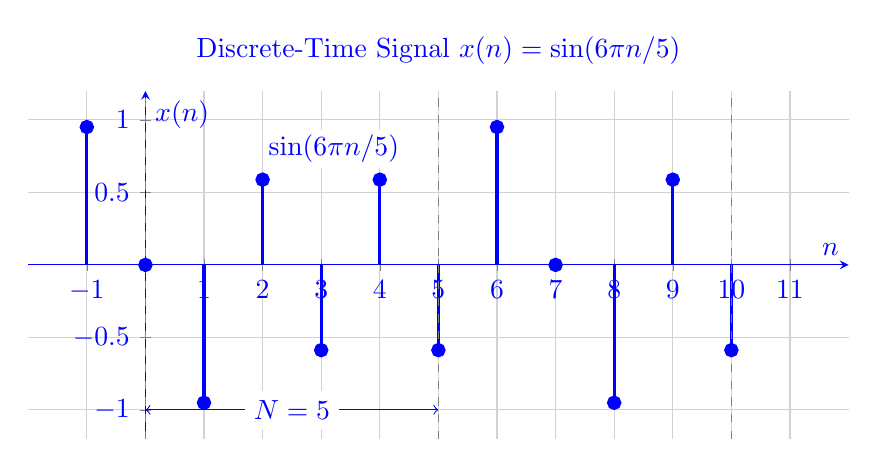
\begin{tikzpicture}
\begin{axis}[
    width=12cm,
    height=6cm,
    axis lines=middle,
    xlabel={$n$},
    ylabel={$x(n)$},
    title={Discrete-Time Signal $x(n) = \sin(6\pi n/5)$},
    xmin=-2, xmax=12,
    ymin=-1.2, ymax=1.2,
    xtick={-1, 0, 1, 2, 3, 4, 5, 6, 7, 8, 9, 10, 11},
    ytick={-1, -0.5, 0, 0.5, 1},
    grid=both,
    grid style={gray!15},
    major grid style={gray!35},
    ycomb, % Discrete-time plot
    mark=*, mark size=2pt, blue,
]

% Plot the discrete-time sinusoidal signal
\addplot[ycomb, blue, very thick, mark=*, mark size=2pt] coordinates {
    (-1, 0.951) (0, 0) (1, -0.951) (2, 0.588) (3, -0.588) (4, 0.588) (5, -0.588) (6, 0.951) (7, 0) (8, -0.951) (9, 0.588) (10, -0.588)
};

% Add period markers
\draw[dashed, gray] (0, -1.2) -- (0, 1.2);
\draw[dashed, gray] (5, -1.2) -- (5, 1.2);
\draw[dashed, gray] (10, -1.2) -- (10, 1.2);

% Add period label
\draw[<->] (0, -1) -- (5, -1) node[midway, fill=white] {$N = 5$};

% Add annotation
\node[anchor=west, fill=white, inner sep=2pt] at (2, 0.8) {$\sin(6\pi n/5)$};

\end{axis}
\end{tikzpicture}

\caption{The discrete-time signal $x(n)$, which is periodic with period $N=5$.}
\label{fig:signal_plot}
\end{figure}
\end{example}

\vspace{0.5em}
\hrule
\vspace{0.5em}
\newpage
\begin{example}[2. DTFS of a Periodic Signal from its Graph]
\textbf{Problem:}
Determine the DTFS coefficients $a_k$ for the periodic signal $x(n)$ shown in Figure \ref{fig:signal}.

\begin{figure}[H]
\centering
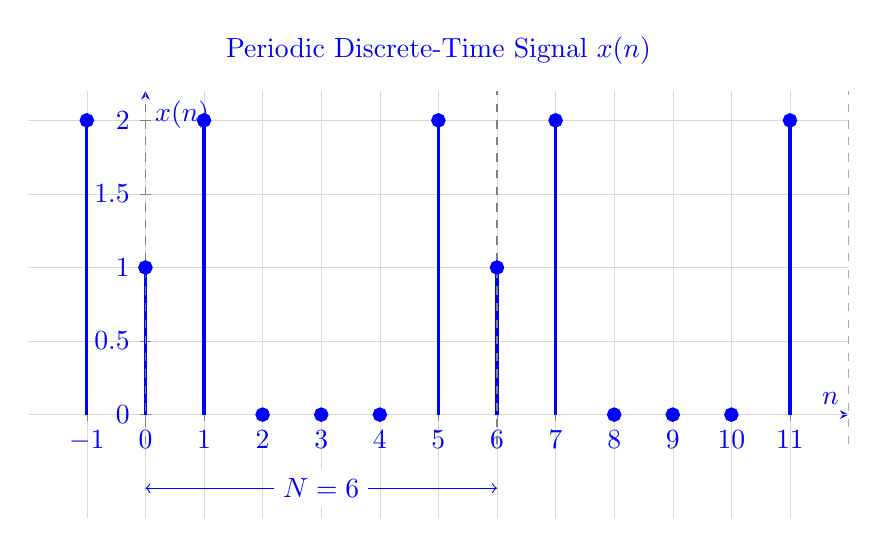
\begin{tikzpicture}
\begin{axis}[
    width=12cm,
    height=7cm,
    axis lines=middle,
    xlabel={$n$},
    ylabel={$x(n)$},
    title={Periodic Discrete-Time Signal $x(n)$},
    xmin=-2, xmax=12,
    ymin=-0.7, ymax=2.2,
    xtick=\empty,
    ytick=\empty,
    extra x ticks={-1, 0, 1, 2, 3, 4, 5, 6, 7, 8, 9, 10, 11},
    extra y ticks={0, 0.5, 1, 1.5, 2},
    grid=major,
    grid style={line width=.1pt, draw=gray!30},
    ycomb, % Discrete-time plot
    mark=*, mark size=2pt, blue,
]

% Plot the periodic discrete-time signal
\addplot[ycomb, blue, very thick, mark=*, mark size=2pt] coordinates {
    (-1, 2) (0, 1) (1, 2) (2, 0) (3, 0) (4, 0) (5, 2) (6, 1) (7, 2) (8, 0) (9, 0) (10, 0) (11, 2)
};

% Add period markers
\draw[dashed, gray] (0, -0.2) -- (0, 2.2);
\draw[dashed, gray] (6, -0.2) -- (6, 2.2);
\draw[dashed, gray] (12, -0.2) -- (12, 2.2);

% Add period label
\draw[<->] (0, -0.5) -- (6, -0.5) node[midway, fill=white] {$N = 6$};

% Add annotation
%\node[anchor=west, fill=white, inner sep=2pt] at (2, 1.5) {Periodic pattern: $[2, 1, 2, 0, 0, 0]$};\\

\

\end{axis}
\end{tikzpicture}

\caption{The periodic discrete-time signal $x(n)$.}
\label{fig:signal}
\end{figure}

\textbf{Solution:}

\textbf{Fundamental period:} $N = 6$

\textbf{DTFS analysis formula:}
$$a_k = \frac{1}{6} \sum_{n=-1}^{4} x(n) e^{-jk(\pi/3)n}$$

\textbf{Non-zero samples:} $x(-1)=2$, $x(0)=1$, $x(1)=2$

$$a_k = \frac{1}{6} \left[ 2e^{jk\pi/3} + 1 + 2e^{-jk\pi/3} \right]$$

$$= \frac{1}{6} \left[ 1 + 4\cos(k\pi/3) \right]$$

\textbf{Answer:}
$$a_k = \frac{1}{6} + \frac{2}{3}\cos\left(\frac{k\pi}{3}\right)$$
\end{example}

\end{document}